\chapter {Produktfunktionen}

\subsection{Grundfunktionen}
\setcounter{counterKriterien}{0}

\subsubsection{Graphische Bedienoberfläche}
% finde es unsinnig pauschal eine Projekterstellungssicht anzuzeigen, vlcht möchte der Benutzer ein
% bereits vorhandenes Projekt öffnen. Das ist mein Vorschlag:
%\nItem{PF} Startbildschirm \\
%Nach dem Start der Anwendung werden dem Benutzer die zuletzt geöffneten Projekte angezeigt. Der Benutzer
%hat dann die Möglichkeit ein bereits bestehendes Projekt zu öffnen oder aber ein neues Anzulegen.
\nItem{PF} Willkommensbildschirm
\newline
Beim Start zeigt die Anwendung einen Willkommensbildschirm an, auf dem allgemeine Informationen und zuletzt
 benutzte Projekte zusammen mit einer \emph{Projekt-Erstellung-Sicht} angezeigt werden.
 % % % % % % % % % % % % % % % % % % % % % % % % % % % % % % % % % % % % % % % % % % % % % % % % % %
 
% Es ist unsinnig zwischen Filtern und Testsignalen zu unterscheiden. Wie soll ein Testsignal aussehen ?
%\nItem{PF} Filtercontainer \\
%Der Filtercontainer ist die Stelle der Grafischen Oberfläche, an der der Nutzer einen, der Anwendung
%zur Verfügung stehenden, Filter auswählen kann (durch einen Klick mit der Maus). Um einen Filter auszuwählen
%muss ein gültiges Video im Projektexplorer gewählt worden sein. Durch die Auswahl eines Filters wird
%der entsprechende Filter als der nächste anzuwendende Filter markiert. Im Visualisierungsbereich des
%Fensters kann der Nutzer alle, in der von ihm gewählten Reihenfolge, markierten Filter und auch den
%dadurch verursachten Effekt sehen. Dem Benutzer steht die Möglichkeit offen einen bereits gewählten
%Filter wieder abzuwählen.
% Man sollte wahrscheinlich erwähnen, dass es nicht möglich sein wird das Video abzuspielen bis der Filter 
% tatsächlich angewandt wurde.
\nItem{PF} Testsignalansicht
\newline
Alle Filter und Testsignale, mit denen eine Referenzdatei manipuliert werden kann, werden aufgelistet. Der
 Benutzer kann beliebige Filter auswählen und nacheinander über einen Button auf eine (im Projektexplorer)
 bestehende Datei anwenden.
% % % % % % % % % % % % % % % % % % % % % % % % % % % % % % % % % % % % % % % % % % % % % % % % % % %

%  Wieder eine in meinen Augen nicht zielführende Unterscheidung zwischen Typen von Videos. 
%  Eine vlcht. geschicktere Version:
\nItem{PF} Projektexplorer \\
Nachdem ein bestehendes Projekt geöffnet oder ein neues erstellt worden ist wird dem
Benutzer, unter anderem, ein Projektexplorer zur Verfügung gestellt. Ein Projektexplorer ist ein 
Fenster das zwei Registerreiter enthält. \\
Der erste Reiter, die Smartlist, enthält die dem Projekt zugewiesenen Videosequenzen. Dabei wird
grundsätzlich zwischen einer Referenz- und Erzeugten Sequenz unterschieden. Wie in Abb.\ref{pExplorer}
ersichtlich ist die Smartlist eine Baumstruktur, dabei ist jedes Vaterelement
ein Referenzvideo im Bezug zu seinen Kindelementen. Beispielsweise ist, in Abb.\ref{pExplorer}, 
">Carphone.yuv"< ein Referenzvideo im Bezug zum Kindelement ">Gaussian Blurr"<. Gaussian Blurr ist ein
vom Nutzer gewählter Name für die Videosequenz ">Carphone.yuv"< an der der Gaußscher Weichzeichner angewandt
wurde und ">processed"< ist der vom Nutzer gewählter Name für die ">Gaussian Blurr"< Videosequenz auf
der er sein \gls{VBW} ausgeführt hat.
\begin{figure}[h]
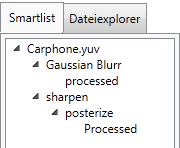
\includegraphics[scale=1]{bilder/projektexplorer.png}
\caption{Projektexplorer}
\label{pExplorer}
\end{figure}
\nItem{PF} Projektexplorer
\newline
Die Anwendung listet alle Referenzvideos und Testvideos des Projekts in einem Projektexplorer auf. Der
 Benutzer kann ein oder mehrere Videos auswählen um auf diesen Filter oder Analysen auszuführen.
% % % % % % % % % % % % % % % % % % % % % % % % % % % % % % % % % % % % % % % % % % % % % % % % % % % % %

\nItem{PF} Darstellung der Analyseergebnisse als Diagramme
\newline
Die Analysedaten werden nach Möglichkeit graphisch durch z.B. Diagramme dargestellt.

\nItem{PF} Darstellung der Analyseergebnisse als Overlay
\newline
Analysedaten (z.B. berechnete Unterschiede) werden als Overlay über dem Video eingeblendet.

\nItem{PF} GUI
\newline
Die Anwendung unterstützt eine interaktive graphische Benutzeroberfläche mit verschiedenen Sichten, die ein-
 und ausgeblendet werden können. Dabei können Ein- und Ausgabevideos abgespielt, sowie einzelne Frames
  ausgewählt und visuallisiert werden.

\subsubsection{Projektverwaltung}
\nItem{PF} Projektverwaltung
\newline
Die Anwendung bietet dem Benutzer die Möglichkeit, durch eine \emph{Projekt-Erstellung-Sicht} Projekte
 anlegen, speichern, löschen und verwalten zu können.

\nItem{PF} Laden von Referenzdateien
\newline
Der Benutzer kann durch ein Dialogfenster eine Referenzdatei im YUV-Format in ein Projekt laden, indem er
 den Pfad zu der Datei angibt. Es können mehrere Referenzdateien geladen werden.

\subsubsection{Portabilität}

\subsubsection{Analyse}

\nItem{PF} Analysewerkzeugsicht
\newline
Alle verfügbaren Analysewerkzeuge werden in dieser Sicht aufgelistet. Der Benutzer kann beliebige Werkzeuge
 markieren und schließlich über einen Button einen Analysedurchlauf für die aus dem Projektexplorer
  ausgewählten Videodateien starten.


\nItem{PF} Analyse-Metriken
\newline
\projektTitel stellt dem Benutzer einige Analyse-Metriken standardmäßig bereit:
\begin{itemize}
\item \gls{MSE}
\item \gls{PSNR}
\end{itemize}


\nItem{PF} Analysedurchlauf
\newline
Wenn ein Analysedurchlauf gestartet wird, werden die ausgewählten Videos mittels der ausgewählten
 Analysemetriken verglichen und die Ergebnisse analysiert, bewertet und optional in eine Logdatei
  gespeichert. Dem Nutzer werden während des Analysedurchlaufs ein Fortschrittsbalken und Statusmeldungen
   angezeigt. 

\subsubsection{Verzerrung}
\nItem{PF} Filter
\newline
Ein Video, welches in ein Projekt eingebunden wurde, kann durch Filter verzerrt werden.Dieses wird
nach dem Verzerren mit ihrem Referenzvideo verknüpft  Auf solch ein verzerrtes Video kann über den Projektexplorer zugegriffen werden um es ggf. weiter zu verzerren oder zu analysieren.


\nItem{PF} Filter-Plugins
\newline
Die Anwendung ist um beliebige Testsignale und Filter in der Form von Plugins erweiterbar.
 Videobearbeitungswerkzeuge (wie z. B. Encoder) kann man auch als externe Filter betrachten und sie als
  Plugins laden, solange sie die Form von ausführbaren Programmen haben und über die Kommandozeile 
angesteuert werden können.

\nItem{PF} Standard-Filter
\newline
Die Anwendung stellt dem Benutzer einige Filter standardmäßig bereit:
\begin{itemize}
\item Weichzeichner
\item Rauschen
\item Farbfilter
\item Blur
\item Schärfe
\item Kantendetektion
\item Emboss
\item Dilatation (Erweiterung)
\item Erosion (Abtragung)

\end{itemize}

\nItem{PF} Generierung von Testdateien
\newline
Wendet man ausgewählte Filter auf eine Datei an, dann wird eine durch die jeweiligen Filter manipulierte Datei im \gls{glos:YUV} Format generiert, die im Projektordner gespeichert und im Projektexplorer bei den Testvideos aufgelistet wird.





\subsection{Optionale Funktionalität}

\nItem{PF} Vorschau für Filter
\newline
Die Auswirkungen eines Filters oder Testsignals auf ein gewähltes Video werden dem Benutzer als Vorschau an einem Frame veranschaulicht.


\nItem{PF} Eingebaute Kommandozeile
\newline
Der Benutzer hat die Möglichkeit, durch eine Kommandozeile Argumente an die Anwendung übergeben zu können.

\nItem{PF} Logdatei
\newline
Es gibt die Option, eine Logdatei für einen Analysevorgang zu erstellen. In der Logdatei sollen im Rahmen
 des jeweiligen Analysevorgangs ausgeführte Operationen sowie erhaltene Ergebnisse in Textformat
  chronologisch aufgelistet werden. Die Auswahl, welche Arten von Operationen und Ergebnissen in der
   Logdatei gespeichert werden sollen, steht dem Benutzer zur Verfügung.
